% Informe de contexto regional de DespachoX, versión corta (máximo 5 páginas).
% Estilo adaptado de prometeo.sty (tesis de Carlos): Ancízar Serif, paleta Sanzo Wada 214, polyglossia.
% Compilar desde docs/informe/:  latexmk -lualatex informe_corto.tex
% El documento de trabajo completo es informe_contexto.tex (versión 0.1).

\documentclass[11pt,letterpaper,parskip=half-]{scrartcl}

% ----------------------------------------------------------------------------- tipografía
\usepackage[no-math]{fontspec}
\usepackage{polyglossia}
\setdefaultlanguage{spanish}
\setmainfont{AncizarSerif}[
  Path=./fuentes/, Extension=.ttf,
  UprightFont=*-Regular, BoldFont=*-Bold, ItalicFont=*-Italic, BoldItalicFont=*-BoldItalic,
  Numbers=OldStyle]
\newfontfamily\ancizarlining{AncizarSerif}[
  Path=./fuentes/, Extension=.ttf,
  UprightFont=*-Regular, BoldFont=*-Bold, ItalicFont=*-Italic, BoldItalicFont=*-BoldItalic,
  Numbers={Lining,Monospaced}]
\newfontfamily\displayfont{AncizarSerif}[
  Path=./fuentes/, Extension=.ttf, UprightFont=*-Light, BoldFont=*-Bold, ItalicFont=*-Italic]
\setmonofont{DejaVu Sans Mono}[Scale=0.80]
\linespread{1.08}
\usepackage[protrusion=true, expansion=false]{microtype}
% Sin patrones de guionado para el español en este sistema: texto en bandera y sin guiones.
\usepackage{ragged2e}
\hyphenpenalty=10000
\exhyphenpenalty=10000
\emergencystretch=2em

% ----------------------------------------------------------------------------- página
\usepackage[letterpaper, top=2.2cm, bottom=2.3cm, left=2.6cm, right=2.6cm, headsep=0.7cm, footskip=1.0cm]{geometry}

% ----------------------------------------------------------------------------- color (Sanzo Wada, combinación 214)
\usepackage{xcolor}
\definecolor{tinta}{HTML}{4F4086}
\definecolor{ambar}{HTML}{A36752}
\definecolor{crema}{HTML}{EBD3A2}
\definecolor{ceniza}{HTML}{6E6878}
\colorlet{noche}{tinta!78!black}
\colorlet{papel}{crema!22!white}
\colorlet{hielo}{tinta!6!white}
\AtBeginDocument{\color{noche}}
\gappto\captionsspanish{\renewcommand{\tablename}{Tabla}}

% ----------------------------------------------------------------------------- títulos (KOMA)
\setkomafont{disposition}{\normalfont\color{tinta}}
\setkomafont{section}{\Large\scshape}
\setkomafont{subsection}{\large\itshape}
\setkomafont{paragraph}{\normalsize\scshape}
\setkomafont{pageheadfoot}{\normalfont\small\color{ceniza}}
\setkomafont{pagenumber}{\normalfont\small\color{tinta}}
\setkomafont{caption}{\small}
\setkomafont{captionlabel}{\small\scshape\color{tinta}}
\RedeclareSectionCommand[beforeskip=-1.2\baselineskip plus -0.3\baselineskip,afterskip=0.35\baselineskip]{section}
\RedeclareSectionCommand[beforeskip=-0.8\baselineskip plus -0.2\baselineskip,afterskip=-0.6em]{paragraph}
\renewcommand*{\sectionformat}{{\color{ambar}\thesection}\enskip}

% ----------------------------------------------------------------------------- encabezados y pies
\usepackage[headsepline=0.3pt]{scrlayer-scrpage}
\clearpairofpagestyles
\ihead{\textsc{Convite · Manizales después del sismo}}
\ohead{\pagemark}
\setkomafont{headsepline}{\color{ceniza!50}}

% ----------------------------------------------------------------------------- tablas, listas, figuras, enlaces
\usepackage{booktabs,tabularx,array}
\AtBeginEnvironment{tabularx}{\ancizarlining}
\newcolumntype{Y}{>{\RaggedRight\arraybackslash}X}
\newcolumntype{L}[1]{>{\RaggedRight\arraybackslash}p{#1}}
\usepackage[shortlabels]{enumitem}
\setlist{itemsep=1pt,topsep=2pt,parsep=0pt}
\usepackage{graphicx}
\usepackage{multicol}
\setlength{\columnsep}{1.2em}
\usepackage{tikz}
\usetikzlibrary{arrows.meta,positioning,calc}
\usepackage[font=small,labelfont={sc,color=tinta},labelsep=period,justification=raggedright,
  singlelinecheck=false,skip=4pt]{caption}
\usepackage{xurl}
\usepackage[colorlinks=true,linkcolor=tinta,citecolor=tinta,urlcolor=tinta,
  pdfauthor={Equipo 19, Convite},pdftitle={Manizales después del sismo: llevar la comida a cada barrio y vereda (versión corta)}]{hyperref}
\urlstyle{same}
\usepackage[most]{tcolorbox}
\tcbset{enhanced,breakable,boxrule=0pt,arc=0pt,outer arc=0pt,left=9pt,right=9pt,top=5pt,bottom=5pt,
  fonttitle=\normalfont\scshape\small,before skip=6pt,after skip=6pt}
\newtcolorbox{propuesta}{colback=papel,colframe=ambar,borderline west={2pt}{0pt}{ambar},
  coltitle=ambar,title={Propuesta en discusión},attach title to upper={\par\smallskip}}
\newtcolorbox{resumen}{colback=hielo,colframe=tinta,borderline west={2pt}{0pt}{tinta},before upper={\setlength{\parskip}{0.3em}}}

% ----------------------------------------------------------------------------- marcas y citas
\newcommand{\marca}[1]{\textcolor{ceniza}{\footnotesize[#1]}}   % [E] evidencia, [I] inferencia, [H] hipótesis
\newcommand{\pv}{\textcolor{ambar}{\textsc{por verificar}}}
\newcommand{\cf}[1]{\textcolor{tinta}{[\ref{#1}]}}                % cita a la lista numerada de fuentes
\newcommand{\cff}[2]{\textcolor{tinta}{[\ref{#1}, \ref{#2}]}}
\newcommand{\horacompilacion}{\directlua{tex.sprint(os.date(string.char(33,37).."H:"..string.char(37).."M", os.time() - 5*3600))}}

\begin{document}
\RaggedRight
\thispagestyle{empty}

% ----------------------------------------------------------------------------- bloque de título
{\small\scshape\color{ceniza} Hackathon UNAL Manizales 2026 · Vertical 04, logística y abastecimiento · Equipo 19\par}
\vspace{0.35\baselineskip}
{\displayfont\fontsize{23}{27}\selectfont\color{tinta} Manizales después del sismo:\\ llevar la comida a cada barrio y vereda\par}
\vspace{0.3\baselineskip}
{\large\itshape Informe de contexto regional de Convite (antes DespachoX). Versión corta para leer y mostrar\par}
\vspace{0.15\baselineskip}
{\color{ambar}\rule{\linewidth}{0.6pt}\par}
{\small\color{ceniza} Viernes 20 de noviembre de 2026, compilado a las {\ancizarlining\horacompilacion}, hora de Colombia. El documento de trabajo completo es la versión 0.1. Marcas: \marca{E} evidencia de la fuente citada, \marca{I} inferencia nuestra, \marca{H} hipótesis por validar, \marca{M} medido por nosotros.\par}
\vspace{0.2\baselineskip}

\begin{resumen}
\textsc{\color{tinta}Resumen.} El sismo del 10 de agosto de 2026 dejó en Manizales 8.240 personas damnificadas, según el censo que cerró el 24 de agosto, y cerró dos de los corredores por los que entra y sale la ciudad. La comida llegó. La red de bancos de alimentos hizo de Manizales uno de sus principales puntos de acopio, pero según Portafolio, el 16 de agosto tenía 404.587 kg en acopio y 157.164 kg en tránsito, y había entregado 41.163 kg. El cuello de botella estuvo en despachar, sobre todo hacia las zonas rurales. En la ciudad, la comida se repartió según las listas del censo y por turnos, en la sede de la Cruz Roja.

Hoy existen piezas sueltas. El Registro Único de Damnificados dice quién es damnificado, la Cruz Roja registra hogares, el sistema SUMA de la OPS lleva inventario y entregas, y la red de bancos recauda y reporta al donante. Ninguna decide qué se manda, a quién, en qué vehículo y por qué vía. Esa es la pieza que propone Convite.

En noviembre la agenda pública de Manizales es la vivienda, y en ciudades con comercio abierto el PMA y la Cruz Roja prefieren el efectivo. Por eso la propuesta en discusión ubica el piloto en la rutina del Banco de Alimentos como nodo regional, con las juntas de acción comunal pidiendo y confirmando, y con la próxima temporada de lluvias como prueba. Ninguna cifra de este informe ha sido verificada todavía por una persona del equipo.
\end{resumen}

% ----------------------------------------------------------------------------- 1
\section{Qué pasó y por qué Manizales es difícil}

El sismo del 10 de agosto de 2026 tuvo magnitud 7,4 y epicentro en San José del Palmar, en el Chocó \cf{f:decreto}. En Manizales, el censo que cerró el 24 de agosto registró 8.240 personas damnificadas y 3.080 predios evacuados. Ese día el Coliseo Mayor seguía como albergue principal \cf{f:censo}.

Las salidas de la ciudad también se cerraron. El 12 de agosto seguían cerrados por completo dos corredores, la vía Pereira–Chinchiná entre los kilómetros 22 y 24 y la vía Manizales–Fresno en Herveo (Tolima), entre los kilómetros 36+800 y 40+300 \cf{f:vias}. No encontramos la fecha en que reabrieron.

\begin{figure}[ht]
\begin{minipage}[b]{0.56\linewidth}
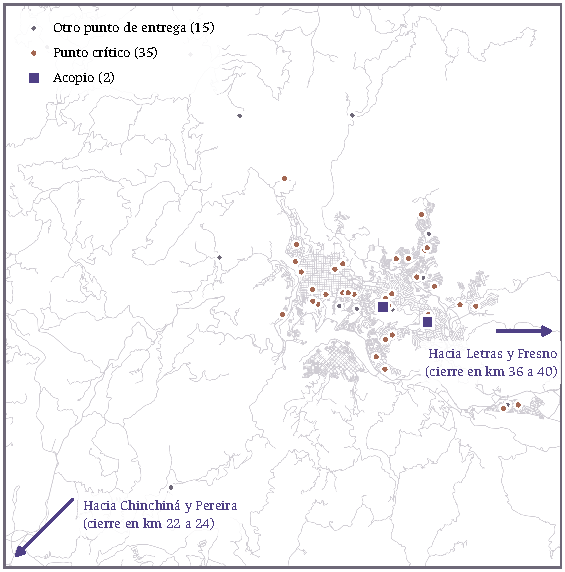
\includegraphics[width=\linewidth]{figuras/mapa_manizales.pdf}
\end{minipage}\hfill
\begin{minipage}[b]{0.41\linewidth}
\caption{Los 50 puntos de entrega del escenario público del equipo, lugares reales con fuente. Hay 35 críticos, como albergues y hospitales, y 15 no críticos. Los cuadrados son los acopios del Banco Arquidiocesano de Alimentos y del Coliseo Menor. Las flechas solo indican la dirección de los corredores cerrados del 10 al 12 de agosto \cf{f:vias}; los cierres quedan fuera del mapa.\newline Red vial: © colaboradores de OpenStreetMap (ODbL).}
\label{fig:mapa}
\end{minipage}
\end{figure}

La geografía explica buena parte de la dificultad. Manizales está sobre una cuchilla y casi todas sus vías de acceso van por ladera (figura~\ref{fig:mapa}), así que los derrumbes las cierran también sin sismo. En marzo de 2021, por ejemplo, un deslizamiento de unos 4.000~m³ cerró la doble calzada a Chinchiná y desvió el tránsito por La Siria \cf{f:ani}. Que la ciudad dependa de pocas vías es inferencia nuestra, porque no hallamos un estudio que lo mida \marca{I}. Al comienzo, además, la región de Caldas, Quindío y Risaralda dejó de recibir el 82~\% de la energía que demandaba \cf{f:decreto}, y sin energía no hay cadena de frío.

El territorio, en cambio, está organizado. Manizales tiene 12 comunas, 7 corregimientos y 204 juntas de acción comunal, 131 en barrios y 73 en veredas \cf{f:jac}. Para Convite esas juntas son la lista natural de quienes piden \marca{I}.

% ----------------------------------------------------------------------------- 2
\section{El cuello de botella fue despachar}

La comida llegó a la región. La red de bancos de alimentos (ABACO) activó un corredor humanitario el 10 de agosto, y Manizales fue uno de sus principales puntos de acopio \cf{f:corredor}. Según la nota del 16 de agosto, sin embargo, la red tenía en acopio y en tránsito mucho más de lo que había entregado (figura~\ref{fig:barras}). La red nombró sus retos el 18 de agosto. El principal fue la llegada al territorio, y le siguieron el transporte, la articulación entre actores, el almacenamiento en los acopios y las vías de acceso hacia las zonas rurales \cf{f:retos}.

\begin{figure}[!ht]
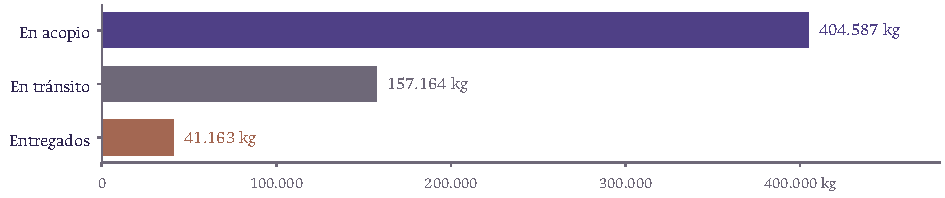
\includegraphics[width=\linewidth]{figuras/barras_abaco.pdf}
\caption{Kilos de la red de bancos de alimentos según Portafolio, 16 de agosto de 2026, seis días después del sismo. La nota no da fecha de corte ni dice si las cifras son nacionales. Fuente: Portafolio, 16 de agosto de 2026 \cf{f:flypass}, citada en la investigación 10 del equipo. Cifras \pv.}
\label{fig:barras}
\end{figure}

En Manizales la comida se repartió según listas. Para recibir mercados en las carpas de atención había que llevar el formato azul que entregan los Bomberos después de revisar la vivienda. La Alcaldía, la UGR y la Cruz Roja entregaron por turnos los kits de alimentos, en la sede de la Cruz Roja Seccional Caldas \cf{f:alcago}. En la Gobernación, la Jefatura de Gestión del Riesgo recibe el requerimiento de cada municipio y deja los kits cargados en el Centro Logístico Humanitario de San Rafael, donde los recogen los vehículos de cada municipio. Al 2 de septiembre llevaba 18.847 unidades entregadas \cf{f:gob}. Nuestra lectura es que el censo y el formato azul definían quién recibía, y el requerimiento municipal definía qué salía del centro departamental \marca{I}. La noche del sismo la Alcaldía pidió no llevar más comida a los albergues, para evitar pérdidas, y desde el 11 de agosto el albergue del Coliseo Mayor dejó de recibir perecederos \cf{f:alcago}.

Hoy la conversación pública es otra. En noviembre, la agenda de la Alcaldía es la vivienda. De 5.591 inmuebles visitados, 2.661 requieren apoyo, y sus notas no mencionan ayuda alimentaria \cf{f:alcnov}. Tampoco hallamos rastro público de despacho de comida del sismo en curso \marca{E}. En ciudades con comercio abierto, además, los grandes operadores prefieren el efectivo. El Programa Mundial de Alimentos (PMA) entregó efectivo en ciudades de Valle y Risaralda y raciones en especie en zonas remotas \cf{f:pma}, y la Cruz Roja planea efectivo multipropósito donde los mercados funcionen \cf{f:dref}. Por eso la comida en especie importa sobre todo en albergues, comedores, instituciones y veredas aisladas \marca{I}.

% ----------------------------------------------------------------------------- 3
\section{¿Hay algo parecido y por qué no se usa aquí?}

\paragraph{Lo que dice la evidencia} Hay piezas sueltas, y cada una sirve a su dueño (figura~\ref{fig:piezas}). El Registro Único de Damnificados (RUD), que consolida la UNGRD, define quién es damnificado y sirve para los subsidios \cf{f:rud}. Cerró el 4 de septiembre y dejó por fuera a familias rurales dispersas \cf{f:vanguardia}. La Cruz Roja registra hogares con AccessRC y, sin señal, con KoboCollect, para focalizar a sus propios beneficiarios \cf{f:dref}. El sistema SUMA/LSS de la OPS lleva inventario y entregas, y Colombia lo adoptó por norma. Sus sitios pueden registrar solicitudes de artículos, pero la página no menciona rutas ni vehículos \cf{f:suma}. La plataforma de ABACO recauda en línea y promete al donante un reporte de entrega, sin asignar vehículos ni rutas \cf{f:donahoy}. Ninguna de las fuentes consultadas describe una herramienta que una pedido, vehículo, vía y entrega \marca{E}.

\begin{figure}[ht]
\centering
% Figura 3 del informe corto: las piezas que existen y la que falta.
% Fuente: docs/investigacion/10_problema_usuarios_alternativas.md, secciones 1 a 3.
% Se incluye con \input desde informe_corto.tex, que define los colores tinta, ambar, ceniza, hielo y papel.
\begin{tikzpicture}[
  font=\small,
  pieza/.style={draw=tinta, fill=hielo, line width=0.6pt, text width=3.2cm, minimum height=1.75cm,
    align=center, inner sep=4pt},
  falta/.style={draw=ambar, fill=papel, dashed, line width=0.9pt, text width=10.2cm, align=center,
    inner sep=6pt},
]
\node[pieza] (rud) at (0,0)
  {{\color{tinta}\textsc{rud}}\\{\footnotesize UNGRD}\\[3pt]{\footnotesize\color{ceniza} quién es damnificado}};
\node[pieza] (kobo) at (4.0,0)
  {{\color{tinta}KoboCollect y AccessRC}\\{\footnotesize Cruz Roja}\\[3pt]{\footnotesize\color{ceniza} registro de hogares}};
\node[pieza] (suma) at (8.0,0)
  {{\color{tinta}\textsc{suma}/\textsc{lss}}\\{\footnotesize OPS}\\[3pt]{\footnotesize\color{ceniza} inventario y entregas}};
\node[pieza] (abaco) at (12.0,0)
  {{\color{tinta}Plataforma de ABACO}\\{\footnotesize red de bancos}\\[3pt]{\footnotesize\color{ceniza} recaudo y reporte al donante}};
\node[falta] (despacho) at (6.0,-2.75)
  {{\color{ambar}\textsc{la pieza que falta: el despacho}}\\[3pt]
   pedido \enspace$\rightarrow$\enspace vehículo \enspace$\rightarrow$\enspace vía \enspace$\rightarrow$\enspace entrega\\[3pt]
   {\footnotesize\color{ceniza}Es lo que propone DespachoX. Una persona aprueba cada plan.}};
\draw[-{Stealth[length=2.6mm]}, ambar, line width=0.9pt]
  (despacho.north -| suma.south) -- node[right, font=\footnotesize, text=ambar] {exporta} (suma.south);
\end{tikzpicture}

\caption{Las piezas que existen y la que falta. Los recuadros morados son herramientas en uso, cada una con su dueño y su fin; el recuadro ámbar es el despacho, que hoy nadie cubre. Elaborado a partir de la investigación 10 del equipo.}
\label{fig:piezas}
\end{figure}

\paragraph{Lo que suponemos} Las razones locales para no usar una herramienta así son hipótesis, porque ninguna fuente pública las documenta \marca{H}. Creemos que pesan el costo del servidor y del soporte, la capacitación, los nombres locales de los lugares y la confianza. También suponemos que la herramienta real de todos es el teléfono, el WhatsApp y la planilla. Inferimos que hoy el Banco, la Alcaldía y la Cruz Roja se coordinan en las reuniones del puesto de mando unificado \marca{I}. Cada supuesto tiene su pregunta en la sección~\ref{sec:nosabemos}.

% ----------------------------------------------------------------------------- 4
\section{¿Quién la usaría?}

El usuario principal que proponemos es el Banco Arquidiocesano de Alimentos de Manizales, porque es un banco de alimentos que opera todo el año y fue nodo del corredor en agosto \cf{f:corredor}. Esa elección es inferencia nuestra y depende de una conversación con el Banco que todavía no ha ocurrido \marca{I}.

\begin{table}[ht]
\small
\renewcommand{\arraystretch}{1.18}
\caption{Quién despacha, quién pide, quién reporta vías y quién decide. La última columna es inferencia nuestra.}
\label{tab:actores}
\begin{tabularx}{\linewidth}{@{}L{1.9cm} Y L{3.3cm} L{3.7cm}@{}}
\toprule
\textsc{Papel} & \textsc{Quién} & \textsc{Con qué trabaja hoy} & \textsc{Qué haría con Convite}\\
\midrule
Despacha & Banco Arquidiocesano de Alimentos, y en Manizales tres camiones de los bancos \cf{f:flypass}; Cruz Roja Seccional Caldas, en cuya sede se entregaron los kits \cf{f:alcago}; Gobernación, hacia los municipios \cf{f:gob} & Censo y formato azul \cf{f:alcago}; AccessRC y KoboCollect; Banco: sin sistema conocido \marca{H} & Plan diario de salidas, lo que vence primero y reporte al donante\\
Pide & 204 juntas de acción comunal \cf{f:jac}, albergues, comedores, hogares de ancianos y municipios y veredas de Caldas & Teléfono, WhatsApp y planillas \marca{H} & Pedido colectivo por junta y confirmación de entrega con QR\\
Reporta vías & Conductores, Policía de Tránsito, concesión vial y socorristas & Teléfono, radio y comunicados & Reporte por chat que recalcula la ruta\\
Decide & Consejo Municipal de Gestión del Riesgo, Unidad de Gestión del Riesgo (UGR) y Alcaldía; Gobernación de Caldas & Actas, censo, RUD y evaluación de daños & Avalar la herramienta en la estrategia municipal de respuesta\\
\bottomrule
\end{tabularx}
\end{table}

% ----------------------------------------------------------------------------- 5
\section{Lo que implica para Convite}

\begin{propuesta}
Propuesta del capitán y del coordinador, hecha con inferencias de las investigaciones 10 y 11 \marca{I}. Ningún aliado la ha visto todavía.
\begin{itemize}[leftmargin=1.2em]
\item \textbf{Rutina del Banco como nodo regional.} El piloto se mediría sobre los despachos de todo el año del Banco Arquidiocesano de Alimentos, hacia organizaciones de Manizales y hacia cabeceras y veredas de Caldas, con un modo de emergencia.
\item \textbf{Marco oficial.} Manizales mantiene la calamidad pública hasta el 9 de agosto de 2027, con un plan de acción específico, según el informe de la Unidad de Gestión del Riesgo al Concejo del 16 de octubre \cf{f:alcnov}. Un piloto de 90 días cabe dentro de ese marco.
\item \textbf{Temporada de lluvias.} Sería la prueba de esfuerzo. En febrero de 2026 la ciudad declaró alerta amarilla por más de 200~mm de lluvia en menos de 25 días \cf{f:lluvia}, el umbral del amarillo del indicador A25 del IDEA de la UNAL, que pasa a naranja desde 300~mm y a rojo desde 400~mm \cf{f:a25}. El A25 ya está en el código como capa de riesgo por tramo, con lluvia de prueba, y en el piloto entraría con datos del IDEA.
\item \textbf{Juntas que piden y confirman.} Las juntas pedirían por su barrio o su vereda sin exigir el RUD, y confirmarían cada entrega con el código QR del paquete. Esas confirmaciones darían al donante el reporte que ABACO ya promete \cf{f:donahoy}.
\item \textbf{Exportación a SUMA.} Recepciones y entregas saldrían en un formato compatible con SUMA, para encajar con el sistema nacional de gestión del riesgo \cf{f:suma}.
\item \textbf{Fases.} Días 0 a 15, acuerdo y línea base. Días 15 a 30, reconstrucción en frío de un mes. Días 30 a 60, un día normal de reparto en paralelo. Días 60 a 90, simulacro con la UGR, A25 por tramo y decisión escrita del Banco.
\end{itemize}
\end{propuesta}

% ----------------------------------------------------------------------------- 6
\section{Lo que no sabemos y a quién preguntar}\label{sec:nosabemos}

\begin{itemize}[leftmargin=1.2em]
\item \textbf{Cómo despacha hoy el Banco Arquidiocesano de Alimentos}, con qué lleva la cuenta de salidas y cómo elige el vehículo. \emph{Al Banco y a ABACO.}
\item \textbf{Cuánta comida se dañó o se venció en agosto}, y dónde. No hay cifra pública. \emph{A la UGR, a la Cruz Roja y al Banco.}
\item \textbf{Si se activó SUMA en agosto}, quién lo opera y qué dice la estrategia municipal de respuesta sobre abastecimiento. \emph{A la UGR.}
\item \textbf{Cuánto duraron los cierres viales} después del 12 de agosto. \emph{A la UGR y a la Policía de Tránsito.}
\item \textbf{Si siguen entregando comida del sismo} y qué albergues siguen abiertos. \emph{Al Banco y a la UGR.}
\item \textbf{Si hubo entregas del PMA en Caldas} y si la Cruz Roja comparte sus registros con la Alcaldía o el Banco. \emph{A la Cruz Roja.}
\item \textbf{Cómo nombra la gente los sitios de entrega} y si las juntas pedirían por este canal. \emph{A líderes de juntas.}
\item \textbf{Cuánto mejora el despacho con velocidades reales.} Con 30 escenarios por nivel de carga y 360 jornadas sobre la red real de Manizales, Convite sube los críticos a tiempo en 23,3, 44,7 y 57,9 puntos frente al despacho por orden de llegada \marca{M}. Cada diferencia compara 30 jornadas por política, y ningún intervalo del 95~\% toca el cero. Frente a un despachador con oficio, recorre 46,0, 56,0 y 42,2 km menos por jornada. En el total de entregas a tiempo empata con carga holgada y media, y con carga alta gana 3,0 puntos. Los perecederos vencidos quedan en 0,0~\%, frente a 1,4~\%, 3,4~\% y 5,6~\% por orden de ingreso, por una regla de bodega que el despachador con oficio también cumple. Priorizar hace esperar al punto peor atendido entre 1,95 y 3,82 horas más que por orden de llegada. Las velocidades son derivadas de mediciones GPS de un bus en Manizales y asignadas por tipo de vía y pendiente (tesis UNAL de 2019, tabla 14, pp. 46 a 48), con 22,6~km/h de media en la ruta de un bus diésel en Manizales (tesis UNAL de 2019, p. 50). La simulación usa la media por tipo de vía. La vida útil no se repitió con lo medido, y la corrida le sigue dando al huevo horas cuando dura días. \emph{Al equipo, antes de citar un resultado.}
\end{itemize}

% ----------------------------------------------------------------------------- fuentes
\section*{Fuentes}
{\footnotesize\ancizarlining
Consultadas el 20 de noviembre de 2026 a través de los informes de investigación del equipo; ninguna ha sido abierta todavía por una persona. La lista completa, con fechas de corte y de consulta, está en el documento de trabajo (versión 0.1).
\begin{multicols}{2}
\begin{enumerate}[label={[\arabic*]}, ref={\arabic*}, leftmargin=2.2em, itemsep=0.5pt]
\item\label{f:decreto} Presidencia de la República. Decreto 1261 de 2026, 19 ago, \href{https://camacol.co/sites/default/files/descargables/DECRETO%201261de%202026_EMERGENCIA_compressed.pdf}{camacol.co}.
\item\label{f:censo} Noticias RCN, 24 ago 2026, \href{https://www.noticiasrcn.com/colombia/manizales-prepara-la-demolicion-de-7-edificios-que-presentan-danos-estructurales-1053593}{noticiasrcn.com}.
\item\label{f:vias} Semana, 12 ago 2026, \href{https://www.semana.com/nacion/articulo/actualizacion-de-las-vias-que-siguen-cerradas-tras-el-terremoto-en-colombia/202602/}{semana.com}.
\item\label{f:ani} ANI, 22 mar 2021, \href{https://www.ani.gov.co/w/se-mantiene-el-cierre-total-de-la-v%C3%ADa-manizales-chinchin%C3%A1-debido-a-las-fuertes-lluvias}{ani.gov.co}.
\item\label{f:jac} Alcaldía de Manizales, consolidado de juntas de acción comunal, 2025, \href{https://manizales.gov.co/wp-content/uploads/2025/08/CONSOLIDADO-JUNTAS-ACCION-COMUNAL-Y-ADMINISTRADORAS-LOCALES-JAC-JAL.pdf}{manizales.gov.co}.
\item\label{f:corredor} Noticias RCN, 10 ago 2026, \href{https://www.noticiasrcn.com/colombia/bancos-de-alimentos-activan-corredor-humanitario-tras-sismo-de-7-4-en-colombia-1048906}{noticiasrcn.com}.
\item\label{f:flypass} Portafolio, 16 ago 2026, \href{https://www.portafolio.co/economia/regiones/flypass-paga-peajes-de-57-camiones-para-acelerar-la-entrega-de-ayudas-tras-el-terremoto-en-colombia-500521}{portafolio.co}.
\item\label{f:retos} Noticias RCN, 18 ago 2026, \href{https://www.noticiasrcn.com/colombia/abaco-supera-las-2-000-toneladas-de-ayuda-humanitaria-recolectadas-para-damnificados-por-el-terremoto-1051306}{noticiasrcn.com}.
\item\label{f:alcago} Alcaldía de Manizales, boletines del \href{https://centrodeinformacion.manizales.gov.co/comunicado-de-prensa-sobre-no-llevar-alimentos-a-los-albergues-por-ahora/}{10}, \href{https://centrodeinformacion.manizales.gov.co/comunicado-de-prensa-sobre-manizales-fortalece-la-atencion-a-las-familias-afectadas-por-el-sismo-en-el-coliseo-mayor-jorge-arango-uribe/}{11}, \href{https://centrodeinformacion.manizales.gov.co/carpas-de-atencion-cable-aereo-y-linea-de-atencion/}{15} y \href{https://centrodeinformacion.manizales.gov.co/alcaldia-ugr-y-cruz-roja-intensifican-entrega-de-auxilios-y-alimentos-a-familias-damnificadas-por-el-sismo/}{31 de agosto de 2026} (centrodeinformacion.manizales.gov.co).
\item\label{f:gob} Gobernación de Caldas, \href{https://escaldas.com/mas-de-8-200-kits-de-ayuda-humanitaria-han-sido-entregados-a-municipios-de-caldas-tras-el-terremoto-del-10-de-agosto/}{18 ago} y \href{https://escaldas.com/gobierno-de-caldas-ha-movilizado-esta-semana-al-menos-6-800-ayudas-humanitarias-ya-completa-mas-de-18-000-entregas-tras-el-sismo/}{2 sep 2026} (escaldas.com).
\item\label{f:alcnov} Alcaldía de Manizales, \href{https://centrodeinformacion.manizales.gov.co/manizales-presento-informe-al-concejo-de-las-acciones-adelantadas-tras-sismo-del-10-de-agosto/}{16 oct 2026}, informe de la Unidad de Gestión del Riesgo al Concejo, y \href{https://centrodeinformacion.manizales.gov.co/manizales-continua-con-los-aportes-para-la-recuperacion-patrimonial-a-propietarios-de-viviendas-y-comerciantes-afectados-por-el-sismo/}{19 nov 2026} (centrodeinformacion.manizales.gov.co).
\item\label{f:pma} Telesur, 19 ago 2026, \href{https://www.telesurtv.net/colombia-onu-asistencia-100000-personas/}{telesurtv.net}.
\item\label{f:dref} IFRC, solicitud DREF MDRCO036, 14 ago 2026, \href{https://go-api.ifrc.org/api/DownloadFile/96426/MDRCO036do}{go-api.ifrc.org}.
\item\label{f:rud} Portafolio, 29 ago 2026, \href{https://www.portafolio.co/economia/gobierno/declaratoria-de-desastre-nacional-por-terremoto-que-cambia-para-colombia-y-como-operara-la-ayuda-501440}{portafolio.co}.
\item\label{f:vanguardia} Vanguardia, 5 oct 2026, \href{https://www.vanguardia.com/colombia/2026/10/05/procuraduria-pide-a-la-ungrd-agilizar-ayudas-para-damnificados-por-el-terremoto/}{vanguardia.com}.
\item\label{f:suma} OPS, sistema SUMA/LSS, \href{https://www.paho.org/es/temas/respuesta-emergencias-salud-desastres/sistema-lss}{paho.org}.
\item\label{f:donahoy} ABACO, plataforma de donación Colombia 2026, \href{https://donahoy.abaco.org.co/colombia2026}{donahoy.abaco.org.co}.
\item\label{f:lluvia} Noticias RCN, 16 feb 2026, \href{https://www.noticiasrcn.com/colombia/declaran-alerta-amarilla-en-manizales-por-lluvias-extremas-992470}{noticiasrcn.com}.
\item\label{f:a25} IDEA-UNAL, registro de lluvias diarias y A25, 2020, \href{https://idea.manizales.unal.edu.co/publicaciones/reportes_meteorologicos/red_manizales/niveles_de_alerta/reportes2020/SAT%20Deslizamientos-Registro%20lluvias%20diarias%20y%20A25%202020.pdf}{idea.manizales.unal.edu.co}.
\end{enumerate}
\end{multicols}
}

\end{document}
